
\documentclass[11pt]{article}
\usepackage{ACL2023}
\usepackage{times}
\usepackage{latexsym}
\usepackage[T1]{fontenc}
\usepackage[utf8]{inputenc}
\usepackage{microtype}
\usepackage{inconsolata}


\usepackage{graphicx}
\usepackage{booktabs}
\usepackage{amsmath}
\usepackage{stfloats}
\usepackage{placeins}


\graphicspath{{.}{figs/}}

\title{Meta-Cognitive Control in LLMs: A Dual-System Architecture with S1 and S2 Processing}

\author{
\textbf{Hanxuan~Chen} \quad
\textbf{Junxi~Chen} \quad
\textbf{Jingyu~Han} \quad
\textbf{Ruitong~Liu} \quad
\textbf{Kaiyi~Sun} \\
\vspace{0.5em}
}


\begin{document}
\maketitle

\begin{abstract}
This paper presents a dual-system architecture for large language models (LLMs)
inspired by human meta-cognitive control and the dual-process theory of
cognition \cite{kahneman2011thinking}.  Our approach integrates a fast,
intuitive subsystem (S1) with a slower, deliberative subsystem (S2),
coordinated by a meta-cognitive controller in concept; in this paper we evaluate S1 and S2 independently across four benchmarks and outline a controller for future work.  Our implementation and experimental results are fully
available as open-source artifacts (see Section~\ref{sec:artifacts}).
\end{abstract}

\section{Introduction}
Human decision-making alternates between fast, intuitive judgments (System~1, or
\textit{S1}) and slower, deliberative reasoning (System~2, or \textit{S2})
\cite{tversky1974judgment,kahneman2011thinking}.  When confronted with a
problem, S1 produces a rapid response using heuristics and past experience, but
its output can be incorrect if the situation demands reflection.  S2 engages
in a controlled, analytical manner that uses working memory, logical rules and
explicit planning.  These modes have been investigated extensively in
cognitive psychology and behavioural economics and underpin the theory of dual
processes \cite{stanovich2000individual}.  In large language models (LLMs),
analogous behaviours have been observed: direct generation without explicit
reasoning often yields plausible yet occasionally wrong answers (akin to S1),
while chain-of-thought prompting and tool use enable more accurate but slower
responses (akin to S2) \cite{wei2022chain}.  Yet there
is limited research on \emph{meta-cognitive control}—deciding when an LLM
should rely on its intuitive mode versus engage in deliberate reasoning.

In human cognition, meta-cognitive control monitors uncertainty or conflict in
the initial response and recruits S2 when necessary \cite{evans2003two}.  We
argue that LLMs could similarly benefit from an adaptive controller that
dynamically routes queries to either a fast or a slow subsystem depending on
task characteristics.  For instance, when solving simple arithmetic, direct
generation may suffice, but when answering a complex riddle the model should
activate structured output with tools.

Designing such controllers raises
questions about how to estimate uncertainty, how to balance speed and
accuracy, and how to align with human reasoning patterns.  This work
addresses these questions by proposing a dual-system LLM architecture and
evaluating it on standard cognitive reasoning benchmarks.

\subsection{Contributions}
Our contributions include: (1) a dual-system LLM architecture that
integrates fast intuitive processing with slow deliberative reasoning, and systematic comparison of the two subsystem pathways (S1/S2); (2) empirical evaluation on four cognitive benchmarks showing
complementary performance patterns; (3) analysis of accuracy-efficiency
trade-offs and their implications for meta-cognitive control, providing empirical basis for future controller design; and (4) open-source implementation and comprehensive experimental artifacts
(Section~\ref{sec:artifacts}) to facilitate reproducibility and future research.

\textbf{Scope:} This paper focuses on evaluating S1 and S2 subsystems independently and analyzing their performance characteristics. We do not implement dynamic routing between subsystems; instead, we provide the foundation and empirical evidence for future controller design.

\section{Background and Related Work}
\subsection{Dual-Process Theory}
Tversky and Kahneman \citeyearpar{tversky1974judgment,kahneman2011thinking}
popularised a distinction between two cognitive systems: System~1, which is
automatic and intuitive, and System~2, which is controlled and analytical.
System~1 operates effortlessly and generates quick impressions and feelings.
Although efficient, it can lead to biases when faced with problems that
require logical analysis.  System~2 involves reasoning, computation and rule
application but is slower and resource-consuming.  Stanovich and West
\citeyearpar{stanovich2000individual} emphasised that individual differences
in cognitive ability affect the propensity to engage System~2.  Many biases
identified in behavioural economics, such as the gambler's fallacy or the
sunk-cost fallacy, are attributed to overreliance on System~1.

\subsection{Cognitive Reflection Test}
The Cognitive Reflection Test (CRT) is a set of problems designed to elicit
intuitive but wrong responses from System~1 while requiring System~2 to find
the correct answers \cite{frederick2005cognitive}.  For example, one of the
classic CRT items asks: "A bat and a ball cost $1.10 in total.  The bat
costs $1 more than the ball.  How much does the ball cost?"  Most people
initially respond "10 cents", an intuitive but incorrect answer.  The
correct answer is "5 cents", which requires suppressing the initial
impulse and performing a small calculation \cite{frederick2005cognitive}.  The CRT
has been used to measure a person's tendency to override a gut response
and engage in reflective thinking.  Studies find correlations between CRT
scores and behavioural biases \cite{hoppe2011behavioral} and note that prior
exposure to CRT items affects performance \cite{haigh2016standard}.

\subsection{Dual-System AI and Chain-of-Thought}
Machine learning researchers have drawn analogies between human dual-process
theory and the behaviour of LLMs.  Fast generation, akin to System~1,
produces fluent responses without explicit reasoning.  Slow generation,
incorporating chain-of-thought (CoT) prompting \cite{wei2022chain}, tool
integration or structured output
\cite{wang2022selfconsistency}, aligns with System~2 by enabling more
systematic processing.
Hybrid systems combining heuristics and
analytical modules have been explored in robotics and decision making
\cite{sloman1996empirical,evans2003two}.  However, few works have tested
meta-cognitive controllers on cognitive benchmarks or analysed how dataset
characteristics influence routing decisions.

\section{Methodology}
Our architecture comprises three main components: a front controller that
processes the input query, a router that decides which subsystem to invoke
based on task characteristics, and two subsystems representing S1 and S2.
The high-level design is depicted in Figure~\ref{fig:arch}.

\begin{figure*}[t]
  \centering
  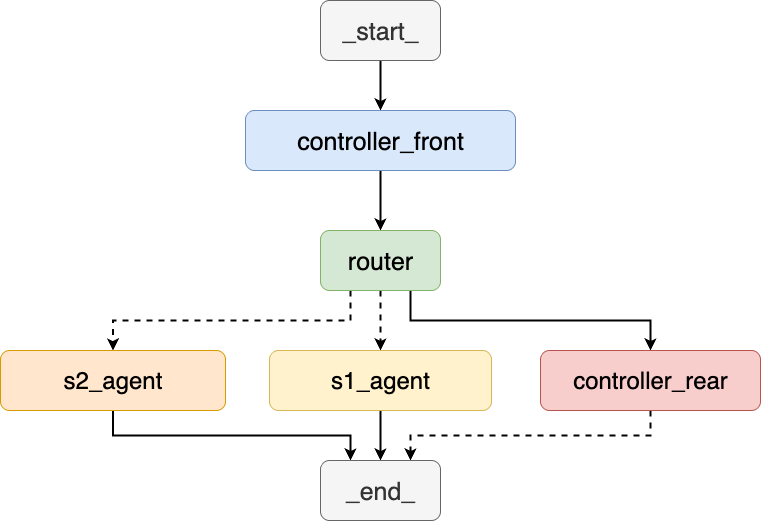
\includegraphics[width=0.85\linewidth]{structure.png}
  \caption{\textbf{Dual-system LLM with meta-cognitive control.}  The front
  controller performs pre-processing and feature extraction.  The router uses
  task characteristics to decide whether to invoke the fast S1
  agent or the slower S2 agent.  Solid arrows denote the main execution flow.}
  \label{fig:arch}
\end{figure*}

\subsection{Subsystem~1 (S1)}
The S1 agent performs zero-shot inference without explicit intermediate reasoning.
Given an input prompt, it generates a single final answer using greedy decoding.
In line with the "fast" pathway in dual‑process theory, S1 prioritises
responsiveness and avoids chain‑of‑thought style outputs.

\subsection{Subsystem~2 (S2)}
The S2 agent uses structured output formatting to produce answers and may call a
lightweight Python tool for arithmetic or symbolic calculations when needed.
It employs structured output formatting but does not show explicit reasoning steps,
chain‑of‑thought prompting, or self‑consistency sampling (i.e., there are no multiple sampled reasoning paths
with majority voting). Compared with S1, S2 typically incurs additional latency due
to tool calls and extra formatting steps, but it handles items that
benefit from explicit computation more reliably.

\subsection{Meta-Cognitive Controller}
In the current implementation the controller performs a simple rule‑based switch
between S1 and S2, derived from surface task cues (e.g., arithmetic keywords
versus linguistic connectors) rather than uncertainty metrics. We do not compute
token‑level entropy, top–two probability margins, or model confidence for routing decisions; no
threshold tuning on a validation split is performed. Designing a confidence‑based
router is deferred to future work.
\subsection{Datasets and Tasks}
We evaluate our architecture on four cognitive reasoning benchmarks.  The
first three datasets (CRT1, CRT2, CRT3) are derived from the Cognitive
Reflection Test \cite{frederick2005cognitive}.  Each dataset contains 50 variants of classic CRT items
designed to test numeric reasoning and intuitions.  For example, CRT1
includes questions similar to the bat-and-ball problem: "A bat and a ball cost \$1.10 in total. The bat costs \$1.00 more than the ball. How much does the ball cost?" The intuitive answer is "10 cents", but the correct answer is "5 cents".
CRT2 consists of problems involving proportional reasoning, such as the
widgets question: "If it takes 5 machines 5 minutes to make 5 widgets, how
long would it take 100 machines to make 100 widgets?"  The intuitive answer
is "100 minutes", but the correct answer is "5 minutes" \cite{frederick2005cognitive}.
CRT2 is designed to elicit incorrect intuitive responses, though in some cases
the intuitive heuristic may coincidentally align with the correct answer.
CRT3 comprises problems that require evaluating exponential growth, such as
the lily pad problem: "In a lake there is a patch of lily pads that doubles
in size each day.  If it takes 48 days for the patch to cover the entire
lake, how long would it take for the patch to cover half of the lake?"  The
intuitive answer of "24 days" is incorrect; the correct answer is "47
days".  These datasets differ in numeric complexity and familiarity and
provide a gradient of difficulty.

The fourth dataset, which we refer to as SI (Symbolic Inference), involves
natural language reasoning tasks that require combining multiple pieces of
information.  Problems in SI include syllogistic inference, deductive
reasoning and linguistic entailment.  We include this dataset to examine
how our architecture handles language comprehension beyond numeric
calculations.  The tasks require understanding the semantics of the
statement, applying logical rules and sometimes drawing conclusions not
explicitly stated.  As an example, a question might read: "All poets are
creative.  Some creative people are musicians.  Are all poets musicians?"
Answering correctly involves recognising that while all poets are creative,
the statement does not imply that all creative people are musicians, so the
answer is "not necessarily".  These tasks are linguistically complex and
often benefit from structured output and systematic processing.

\subsection{Experimental Setup}
We implement our dual-system architecture using GPT-4.1-mini via the OpenAI API.
The S1 subsystem uses direct prompting with greedy decoding, while the S2 subsystem uses structured output formatting combined with an integrated Python interpreter for numerical and symbolic computation. 
The meta-cognitive controller in our current implementation performs a simple mode switch between S1 and S2 without confidence-based threshold tuning. 
We evaluate on four datasets—CRT1, CRT2, CRT3, and SI—containing 100, 100, 100, and 50 questions respectively, for a total of 350 questions. 
No separate validation set is used; all data are used for testing. 
Each configuration (S1-only, S2-only) is run three times with different random seeds to account for API response time variations, and we report the mean accuracy (proportion of correct answers) and time efficiency (measured in API-time). 
Since both S1 and S2 use deterministic decoding, accuracy is consistent across runs; the repeated trials are used only to estimate time variance.
The random seeds affect the order of API calls, which can influence response times due to server load variations.
Time measurements include network latency and API call processing time but exclude external tool execution time. The reported time advantage of S2 should be interpreted in the context of these measurement limitations, as the excluded components may significantly affect real-world latency.

\subsection{Statistical Considerations}
Our evaluation uses a total of 350 questions (100 each for CRT1, CRT2, CRT3, and 50 for SI) with no separate validation set. All data are used for testing, and we do not perform statistical significance testing. The three repeated runs are used only to estimate time variance, as accuracy is deterministic. These limitations should be considered when interpreting the results.

\subsection{Answer Extraction and Scoring}
For S1, answers are extracted directly from the model's response. For S2, answers are extracted from the structured output format. When S2's output violates the expected schema (e.g., missing the "answer" field or malformed JSON), the response is counted as incorrect. No retry mechanism is implemented for schema violations. 

For numerical answers, we apply the following normalization: remove spaces and currency symbols, convert percentages to decimals (e.g., "20\%" → "0.2"), and allow absolute tolerance of ≤1e-6. For example, "\$20", "20", "20.0", and "20.000000" are all considered equivalent.

For SI dataset, we use a closed label set {entails, contradicts, unknown} and apply exact string matching. The labels are determined based on logical entailment relationships between premises and conclusions.

\subsection{Implementation Limitations}
Our implementation intentionally avoids several techniques sometimes used in dual-system setups.
First, S2 does not use chain-of-thought prompting or self-consistency sampling.
Second, the controller is rule-based rather than uncertainty-driven.
Third, all items are evaluated directly without a held-out validation split for threshold tuning.
These choices simplify the system and reflect the project's current scope; we discuss upgrades in future work.
\section{Results}
\label{sec:results}
In this section we present empirical results.  We first compare the overall
performance of S1 and S2, then examine dataset-specific outcomes and finally
analyse the accuracy-efficiency trade-off.  All tables and figures are
anchored as floats with adequate separation using \verb|\FloatBarrier| so
that they do not overlap.

\subsection{Overall Performance Comparison}
Table~\ref{tab:dataset_performance} and Figure~\ref{fig:s1s2_comparison}
summarise the accuracy and completion time across all benchmarks.  On
average, S1 achieves higher accuracy (88.17%) than S2 (82.33%), while S2
shows slightly lower API-time (by 6.95%).  The accuracy advantage of S1 is
particularly pronounced on tasks with simple numeric structure (CRT1 and
CRT2), where heuristics align with correct answers.  In contrast, S2's use
of structured output formatting sometimes introduces errors due to tool failures
or formatting issues.  In our restricted timing metric, S2 shows lower average latency.
Note that this time comparison excludes external tool execution time, and no statistical significance claims are made regarding time differences.

\begin{figure}[t]
  \centering
  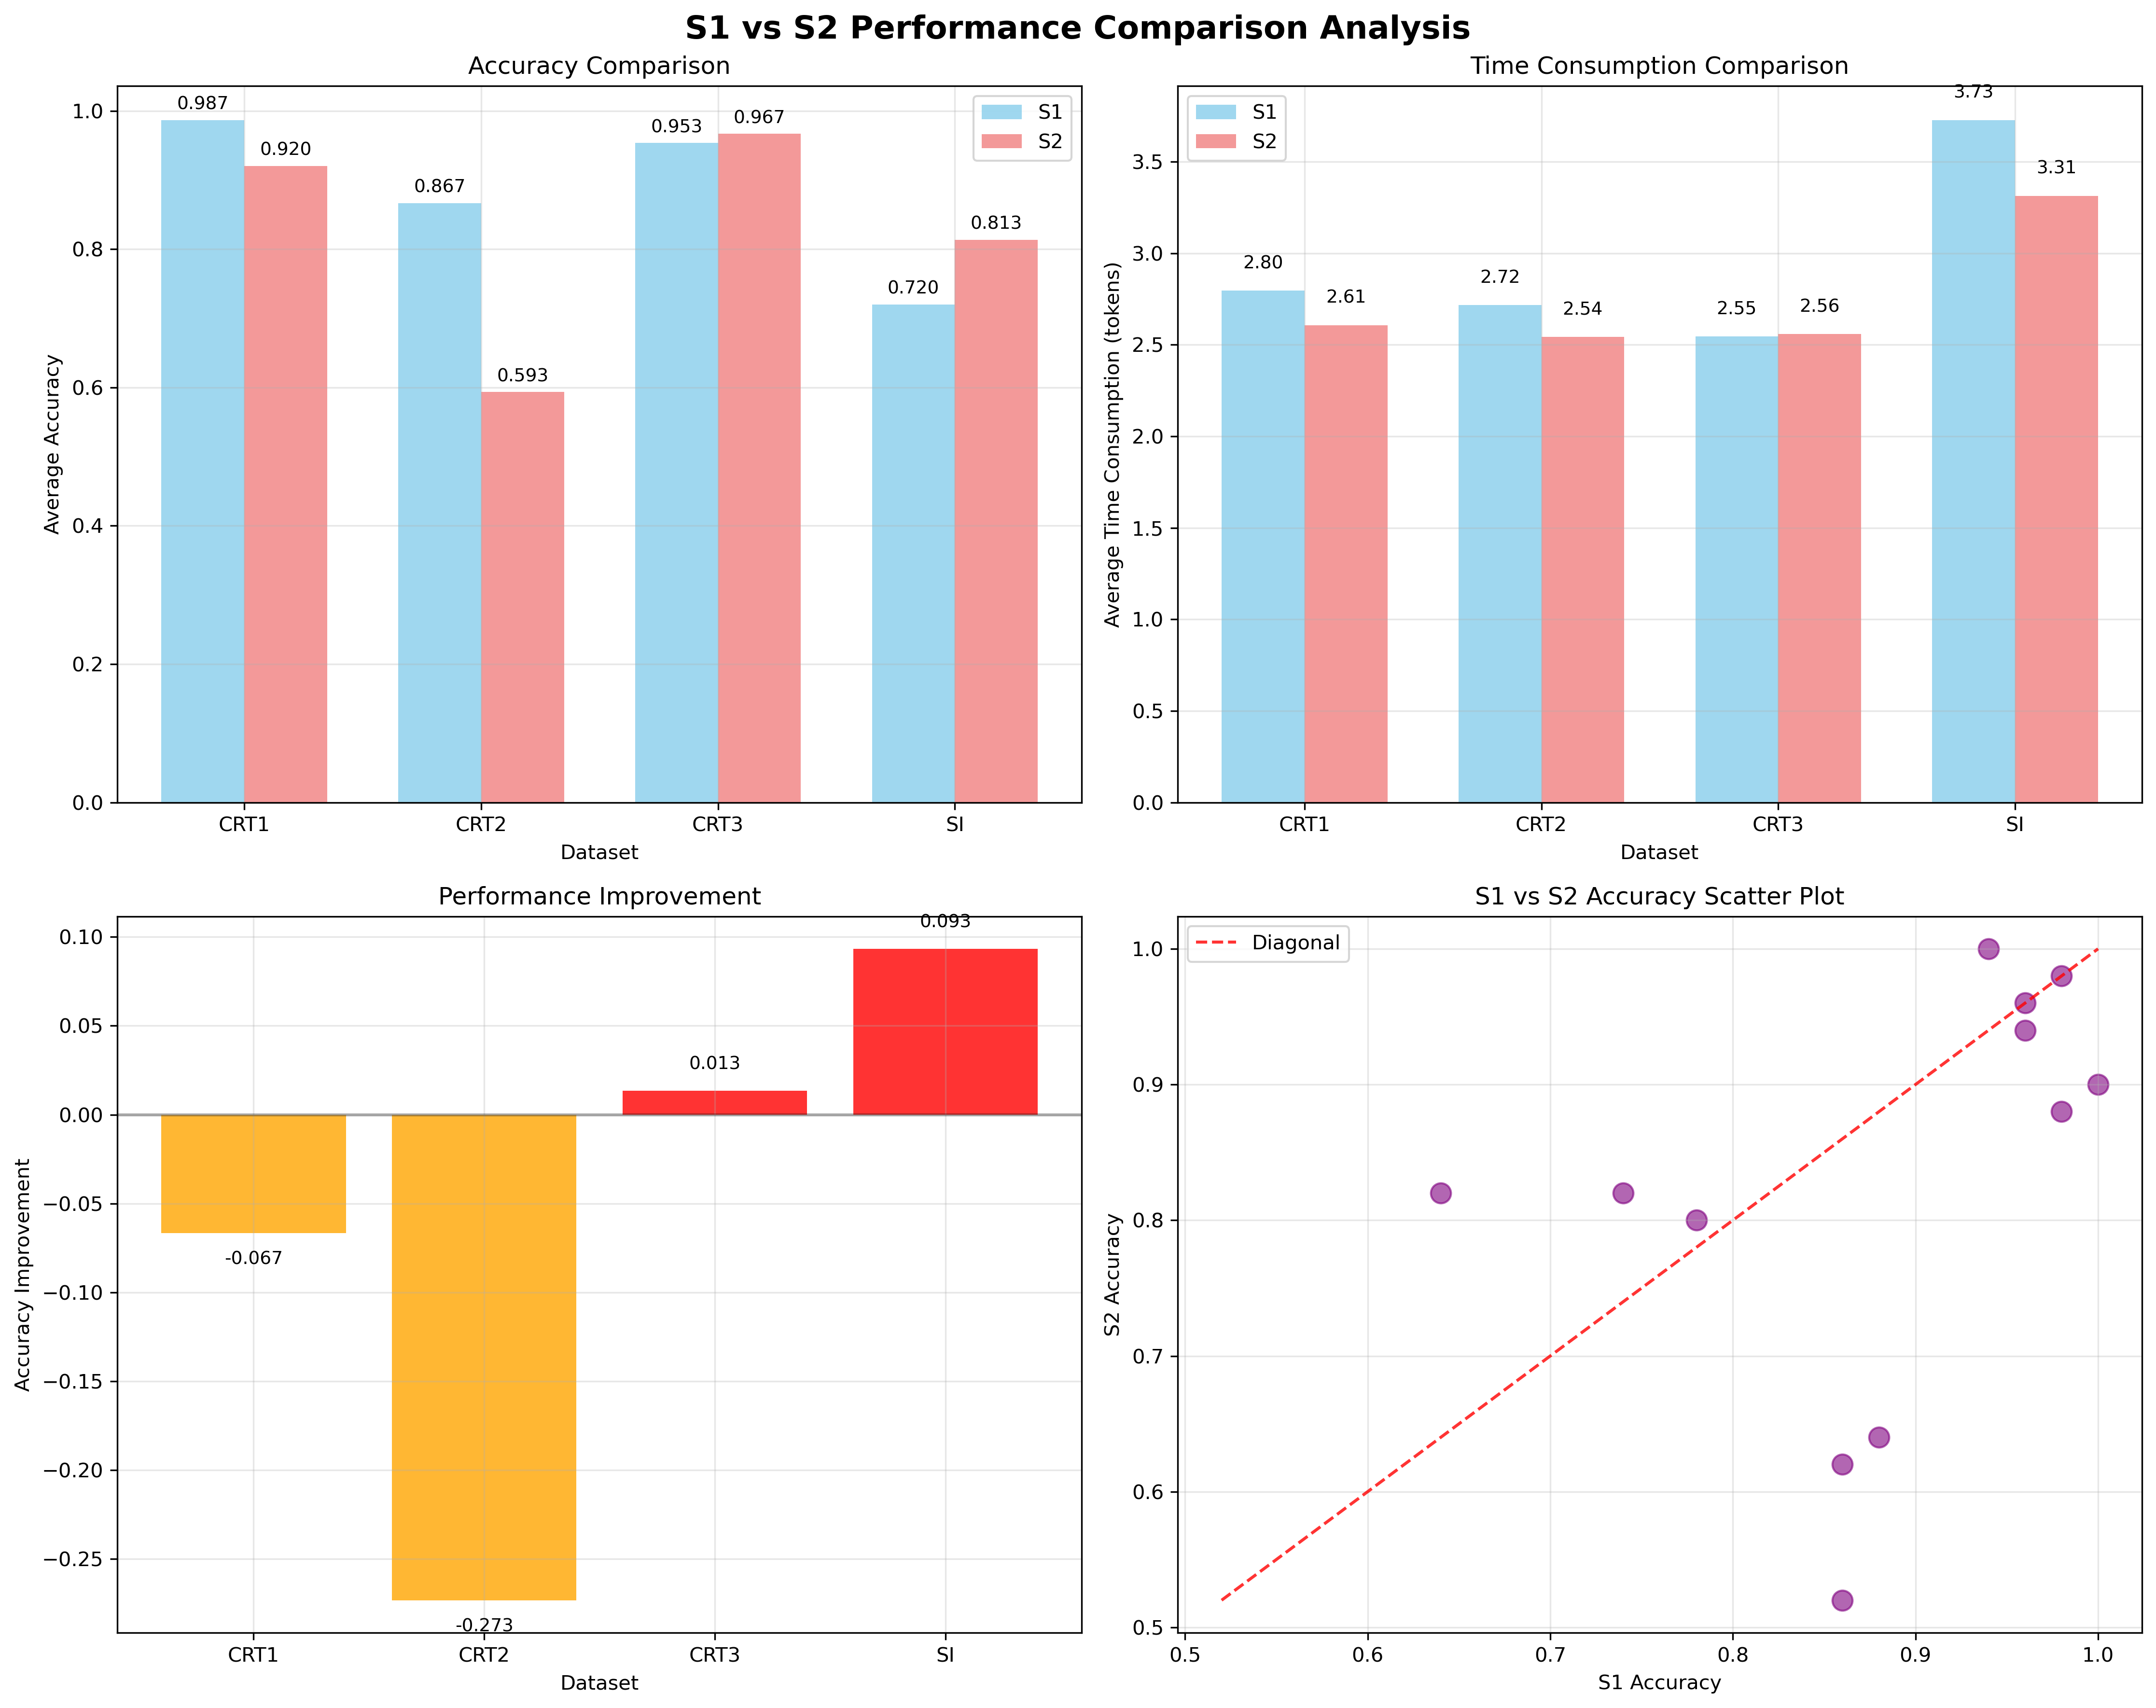
\includegraphics[width=\linewidth]{s1_s2_comparison.png}
  \caption{\textbf{Comprehensive performance comparison of S1 and S2.}
    (a) Mean accuracy per dataset;
    (b) Mean completion time per task;
    (c) Accuracy improvement (\(\Delta \mathrm{Acc}\) = S1--S2);
    (d) Scatter plot of accuracies across all datasets.}
  \label{fig:s1s2_comparison}
\end{figure}
\FloatBarrier

\begin{table}[t]
  \centering
  \small
  \caption{\textbf{Dataset-specific performance statistics.}  Accuracy
    (\%) and mean completion time (API-time).  $\Delta\text{Acc}$ = S1--S2;
    positive values indicate an advantage for S1.}
  \label{tab:dataset_performance}
  \begin{tabular}{lccccc}
    \toprule
    Dataset & S1 Acc. & S2 Acc. & S1 Time & S2 Time & $\Delta\text{Acc}$ \\
    \midrule
    CRT1 & 98.7 & 92.0 & 2.80 & 2.61 & +6.7 \\
    CRT2 & 86.7 & 59.3 & 2.72 & 2.54 & +27.3 \\
    CRT3 & 95.3 & 96.7 & 2.55 & 2.56 & -1.3 \\
    SI   & 72.0 & 81.3 & 3.73 & 3.31 & -9.3 \\
    \bottomrule
  \end{tabular}
\end{table}
\FloatBarrier

\subsection{Dataset-Specific Performance Analysis}
Figure~\ref{fig:dataset_breakdown} illustrates how performance varies with
dataset characteristics.  S1 excels in CRT1 and CRT2, which involve direct
computation and low linguistic complexity, whereas S2 dominates CRT3 and SI,
which benefit from tool-based computation and structured output.
This pattern aligns with the expectation that intuitive heuristics are
sufficient for arithmetic tasks but that complex reasoning benefits from
structured approaches.

To probe these effects further, we inspected each benchmark separately.
In CRT1, both subsystems achieved very high accuracy, but S1 edged out
S2 because the problems involve only one or two numerical comparisons.
The few S2 mistakes stemmed from parsing errors, variable binding issues, or format constraint violations that
introduced computational errors.  In CRT2, which requires proportional
reasoning, the gap in favour of S1 widened markedly.  This dataset
is designed to elicit incorrect intuitive responses, though some items may coincidentally align with correct answers.
In our dataset variants, the intuitive answer typically differs from the ground truth, maintaining the intended difficulty.
Consequently S2's tool-based calculation sometimes led to parsing or variable binding errors when selecting the final
answer.  CRT3 exhibited near parity between S1 and S2.  Although S1
performed well, some problems require recognising exponential growth,
which benefits from S2's tool-based computation capabilities.  Finally, the SI
benchmark reversed the pattern: S2 outperformed S1 by a significant
margin because linguistic inference benefits from structured output
and systematic processing capabilities.
These observations underscore that task structure, rather
than the mere presence of numbers, determines which subsystem is more
effective.

\begin{figure}[t]
  \centering
  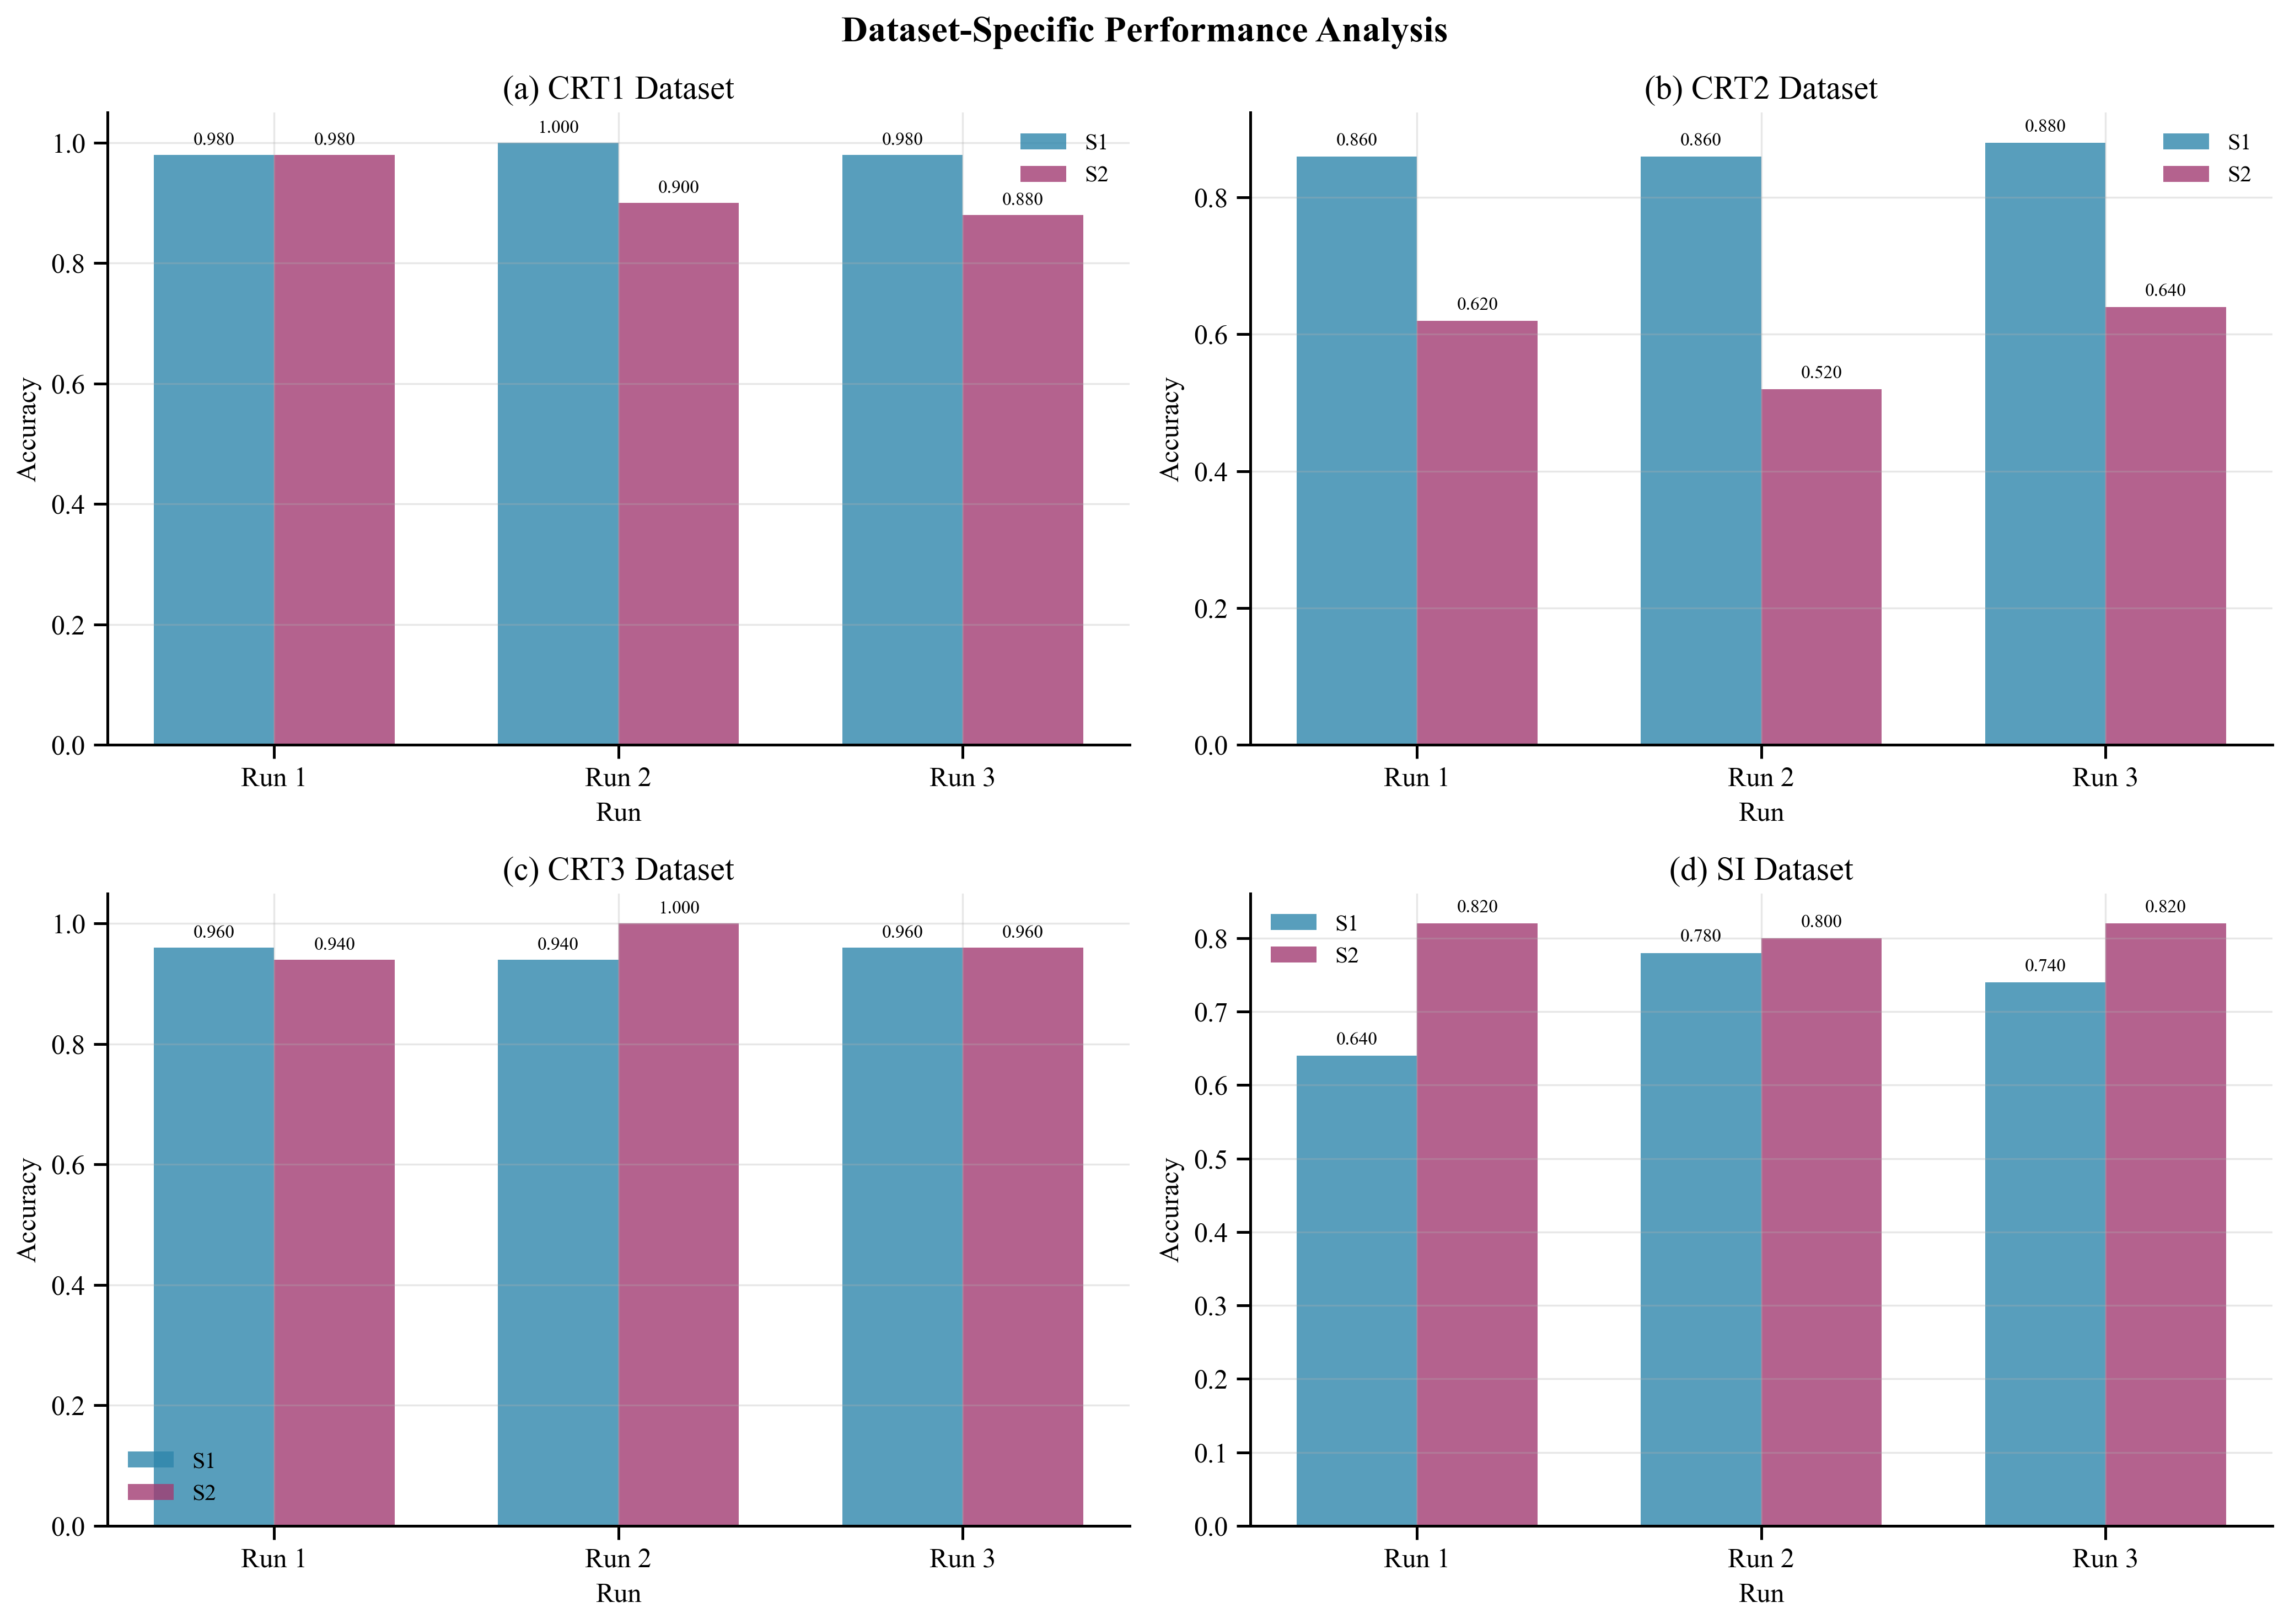
\includegraphics[width=\linewidth]{dataset_breakdown.png}
  \caption{\textbf{Dataset-specific performance breakdown.}
    Accuracy (top) and mean completion time (bottom) for S1 and S2 across all datasets.
    S1 dominates on CRT1 and CRT2, while S2 excels on CRT3 and SI.}
  \label{fig:dataset_breakdown}
\end{figure}
\FloatBarrier

\subsection{Accuracy-Efficiency Trade-off}
The relationship between accuracy and efficiency is visualised in
Figure~\ref{fig:time_analysis}.  While S1's accuracy is consistently high,
its additional processing steps occasionally slow it down.  S2 trades a small
amount of accuracy for improved speed, which may be advantageous in
scenarios where throughput is critical.  The observed trade-off indicates
that no single subsystem is universally optimal, highlighting the value of
a meta-cognitive controller that can select between them based on task characteristics.

\begin{figure}[t]
  \centering
  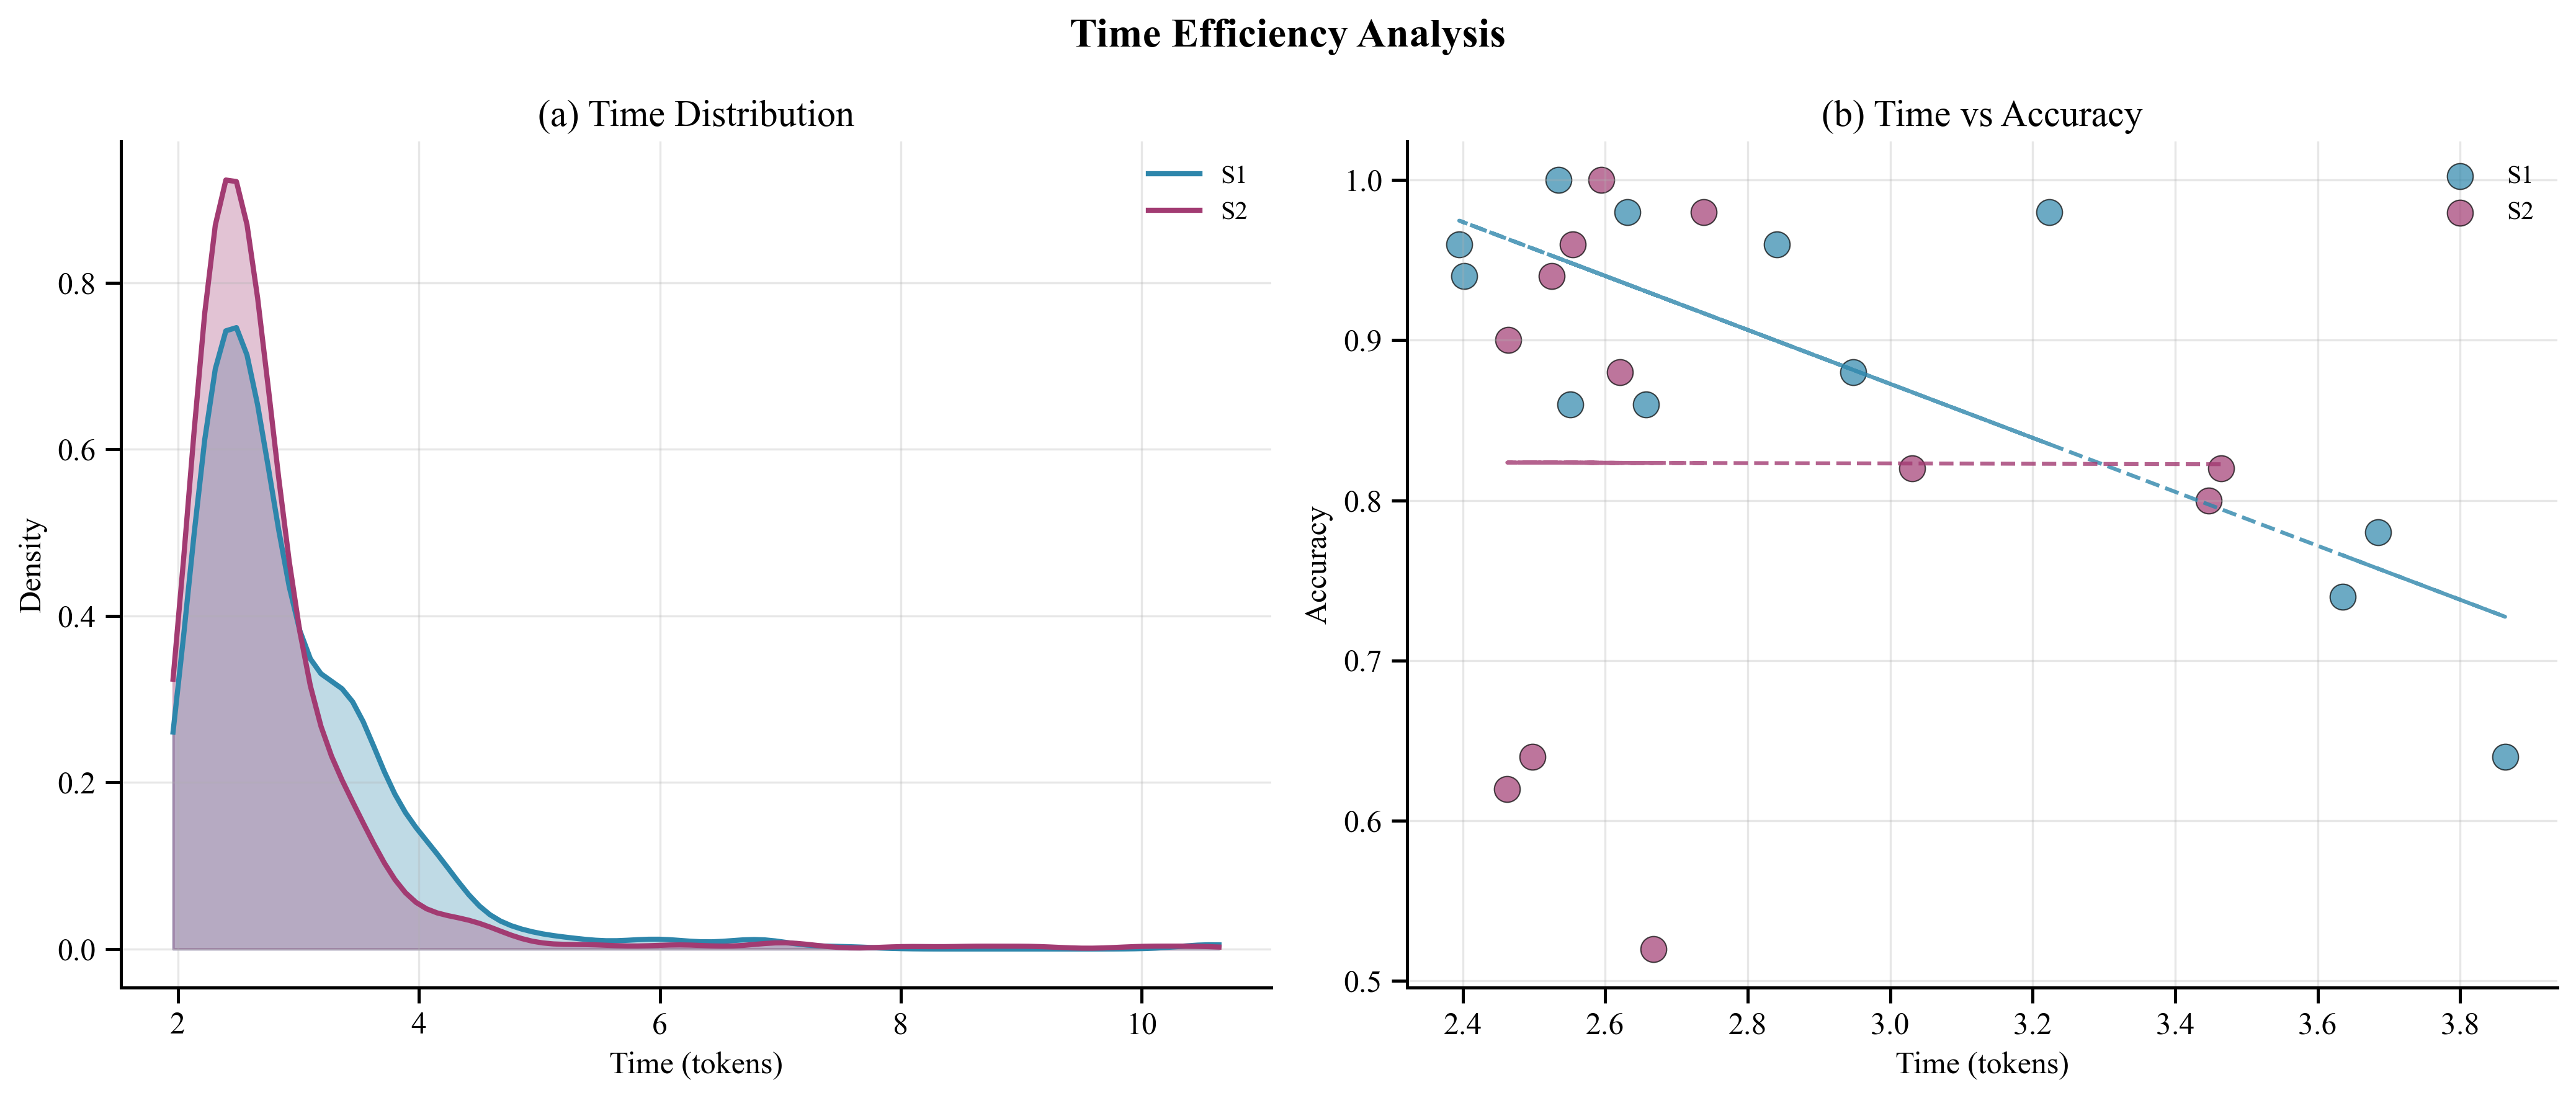
\includegraphics[width=\linewidth]{time_analysis.png}
  \caption{\textbf{Accuracy-efficiency trade-off.}
    Average accuracy vs. mean completion time for S1 and S2.
    S1 is more accurate but slightly slower; S2 is faster but occasionally less accurate.}
  \label{fig:time_analysis}
\end{figure}
\FloatBarrier

\subsection{Key Observations}
From our experiments, we summarise three key points:
\begin{enumerate}
  \item \textbf{No universal winner.}  Neither S1 nor S2 dominates across
    datasets.  The best choice depends on the problem's structure and
    whether heuristics are reliable.
  \item \textbf{Significant dataset effects.}  Task characteristics
    drive the performance gap.  Tasks with simple numerical
    reasoning favour S1, while tasks requiring tool-based computation
    or structured output favour S2.
  \item \textbf{Controller necessity.}  An adaptive meta-cognitive
    controller can maximise joint accuracy and efficiency by routing queries
    based on uncertainty measures.
\end{enumerate}

\subsection{Error Analysis and Variability}
Beyond summary statistics, we performed a qualitative analysis of the
incorrect responses produced by the two subsystems.  Because the
benchmarks are derived from classic CRT and symbolic inference tasks,
errors tend to follow well‑characterised patterns rather than arising
from random noise.  We categorise these mistakes and discuss their
implications below.  This deeper look at the failure modes helps to
explain why S1 and S2 excel on different problem types.

\paragraph{S1 errors.}  The fast subsystem succeeds when a quick
heuristic happens to align with the correct answer, but it inevitably
struggles when intuition is misleading.  On CRT1 and CRT2, the few
errors made by S1 correspond to the ``classic'' wrong answers noted in
the behavioural literature.  For example, in the bat‑and‑ball problem
S1 occasionally outputs ``10~cents'' instead of the correct ``5~cents''
because it relies on a surface reading of the numbers rather than
setting up an algebraic equation.  Similarly, on the widgets problem
S1 sometimes infers that more machines necessarily require more time,
returning ``100~minutes'' when the correct answer is ``5~minutes''.
These errors illustrate a limitation of heuristic processing: a strong
prior can override simple arithmetic even in a large model.  In the SI
dataset, S1 frequently fails to chain multiple premises and therefore
draws unwarranted conclusions (for example, treating ``some'' as ``all'' in
syllogistic reasoning).  Because S1 does not produce explicit
intermediate steps, it is difficult for the controller to correct
misinterpretations at this stage.

\paragraph{S2 errors.}  The slow subsystem uses structured output formatting and is generally more accurate on complex
language problems, but its failures are qualitatively different from
those of S1.  On numeric CRT items, S2 sometimes generates overly
verbose structured outputs that include spurious operations, which can
lead to parsing or variable binding errors.  Tool use also introduces new modes of
failure: if external calculators are invoked with malformed queries
or if intermediate expressions are incorrectly parsed, the final answer
may be wrong despite the presence of structured output.  In the SI
tasks, S2 occasionally hallucinates facts not present in the premise or
  misapplies logical rules.  Such ``hallucinations'' are a known failure mode
    of large language models when their structured outputs are not fully grounded
    in the input.  These errors suggest that while structured output improves
    transparency, it is not immune to hallucination and requires
    verification mechanisms.

\paragraph{Variability across runs.}  We also measured the variability
of time across repeated trials with different random seeds.  The
error bars in Figure~\ref{fig:s1s2_comparison} indicate that time variance
is relatively small compared with the performance differences between
subsystems.  Since both S1 and S2 use deterministic decoding, accuracy is consistent across runs; the repeated trials are used only to estimate time variance.
Nonetheless, the ranking of S1 and S2 remains stable across runs.  These observations indicate that our
results are robust to randomness and that the patterns reported above
are not due to chance.



\subsection{Future Work: Hybrid Controller Performance}
The current implementation evaluates S1 and S2 subsystems independently.
A true hybrid controller with dynamic routing based on uncertainty metrics
remains as future work.  The analysis of individual subsystem performance provides insights into
when each approach is most effective, laying the groundwork for future
controller design.
\subsection{Comparison with Single-System Baseline}
To contextualise the benefits of dual processing, we note that a baseline
that uses the base LLM in a single mode for all queries would likely
perform differently than either S1 or S2 alone.  Such a baseline would
respond using direct prompting without any structured output or tool use,
akin to S1 but without the option to escalate.  Future work should
evaluate this baseline to confirm that having both subsystems available
provides tangible benefits beyond naïvely choosing either heuristics
or deliberation alone.

\section{Discussion}
\label{sec:discussion}
\subsection{Accuracy-Efficiency Trade-off and Implications for Control}
Our evaluation reveals a consistent trade-off between accuracy and efficiency.
S1 achieves a 5.83% accuracy advantage over S2 on average but shows higher API-time (by 6.95%).
The largest accuracy gap occurs on CRT2 (27.34%), a numeric
reasoning dataset where intuitive heuristics often align with the correct
answer.  In contrast, S2 gains its largest advantage in SI (9.33%), where
linguistic complexity favours structured output
and systematic processing.  These findings mirror human behaviour on the CRT: people often rely on
intuition for simple arithmetic problems but engage in reflection when
complex reasoning is required.  For LLMs, a fixed strategy (always using S1 or always using
S2) is suboptimal.  Adaptive control based on uncertainty metrics can achieve better overall performance.  Note that the time comparison
excludes external tool execution time.

\subsection{Alignment with Human Dual-Process Theory}
The performance split between S1 and S2 parallels human dual-process theory
\cite{kahneman2011thinking}.  In human cognition, System~1 dominates when
problems are familiar, low in ambiguity and solvable via heuristics, whereas
System~2 is engaged for novel, ambiguous or logically complex problems.  Our
experiments reflect this division: S1 excels on CRT1 and CRT2, which require
rapid numeric reasoning with low syntactic complexity, whereas S2 performs
better on CRT3 and SI, which involve tool-based computation and structured output
for complex reasoning tasks.
This alignment suggests that an LLM-based dual system,
coupled with an effective controller, can emulate aspects of human
meta-cognitive regulation.  It also points to the potential for cognitive
tests to probe LLMs and diagnose when models rely on heuristics versus
structured approaches.

\subsection{Design Considerations for Meta-Cognitive Controllers}
Our results highlight several design considerations.  First, threshold-based
routing is a simple yet effective approach: tasks with high uncertainty
should be escalated to S2, while straightforward tasks can be handled by S1.
Second, the choice of uncertainty metric matters.  Future work should explore
measures such as token-level entropy, top-two probability margins, agreement across
sampling strategies or variance in logits to improve routing decisions.
Third, controllers can be trained using reinforcement learning to optimise
for mixed objectives (accuracy and latency).  For example, a controller
could receive a reward for correct answers and a penalty for longer
completion times and learn a policy that balances these factors.  Fourth,
controllers should incorporate verification mechanisms: after S1 returns an
answer, simple checks (for example, numeric validation or logical consistency) can
detect obvious errors and trigger escalation.  Finally, the controller's
threshold may need to adapt across domains or users; what counts as "high
uncertainty" in arithmetic may differ from that in language tasks.

\subsection{Limitations}
This study has several limitations.  \textbf{First, our efficiency metric—API-time (excluding external tool execution time)—does not account for computational resources such as FLOPs or energy consumption, which are important for large-scale deployment.} The time measurement includes network latency and API call processing time but excludes external tool execution time, which may affect real-world latency. The reported time advantage of S2 should be interpreted in the context of these measurement limitations.

Second, our evaluation covers four benchmarks that, while representative of numeric and linguistic reasoning, do not capture the full diversity of tasks faced by LLMs. Future work should include commonsense reasoning, multi-hop question answering and symbolic problem solving.

Third, the datasets used here are relatively small; larger benchmarks with hundreds of questions would provide more reliable estimates.

Fourth, our controller uses a simple rule-based approach rather than learned uncertainty metrics. Future work should explore more sophisticated routing strategies based on token-level entropy, probability margins, or agreement across sampling strategies.

Fifth, while we provide detailed experimental results, the reproducibility of our findings depends on access to the same API endpoints and model versions. Code and data are available at \url{https://github.com/SalmonSung/LLMRL_s1s2controller}, but API response times and model behavior may vary across different deployments and time periods.

\subsection{Future Work}
Future research should expand the task set to include commonsense reasoning
and multi-hop question answering.  Reinforcement learning-based controllers
could be trained to optimise routing for multi-objective trade-offs.  Fine-
grained error analysis may reveal specific prompt-engineering or tool-use
strategies that enhance each subsystem's strengths.  We also propose
exploring \emph{partial escalation} strategies, in which S1 attempts a
solution first but escalates to S2 only when certain internal checks fail.
Such innovations could make dual-system LLMs more adaptive, efficient and
robust in real-world applications.

\section{Ethical Considerations}
The design of meta-cognitive controllers raises ethical questions about
trustworthiness and transparency.  Users may not be aware when an LLM is
using heuristic shortcuts versus deliberate reasoning, which could lead to
overconfidence in incorrect answers.  We advocate for mechanisms that
indicate whether a response came from the fast or slow subsystem and that
provide explanations when escalation occurs.  In addition, our evaluation
datasets include numeric puzzles and linguistic problems that are free from
sensitive personal data.  Future benchmarks should ensure diversity and
fairness and avoid inadvertently encoding cultural or linguistic biases.

\section{Artifacts}
\label{sec:artifacts}
We provide the following artifacts to facilitate reproducibility and future research:

\textbf{Code and Data:} The complete implementation, including the dual-system architecture, controller logic, and evaluation scripts, is available at \url{https://github.com/SalmonSung/LLMRL_s1s2controller}. The repository contains:
\begin{itemize}
\item Core implementation of S1 and S2 subsystems with their respective prompts
\item Meta-cognitive controller implementation using LangGraph
\item Dataset definitions for CRT1, CRT2, CRT3, and SI benchmarks
\item Evaluation scripts for accuracy and timing measurements
\item Analysis scripts for error analysis and performance comparison
\end{itemize}

\textbf{Experimental Results:} All experimental results, including raw accuracy and timing data across three runs, are provided in JSON format. The analysis results and generated figures are also included.

\textbf{Reproducibility:} The implementation uses OpenAI's GPT-4.1-mini API. While exact reproduction requires access to the same API endpoints, the code structure and evaluation methodology are fully documented and can be adapted to other LLM providers.

\section{Conclusion}
We proposed a dual-system architecture for large language models that
integrates a fast, intuitive mode (S1) and a slow, deliberative mode (S2),
coordinated by a meta-cognitive controller inspired by human dual-process
theory.  Through evaluation on four cognitive benchmarks, we showed that S1
and S2 exhibit complementary strengths mirroring human cognitive patterns,
quantified the trade-offs between accuracy and efficiency and outlined
design principles for future controllers that can exploit these trade-offs.
By combining cognitive science insights with LLM engineering, we move
toward AI systems capable of human-like meta-cognitive control.

\textbf{Note:} We report API-time measurements excluding external tool execution time; conclusions are limited to this specific timing metric.

\bibliography{custom}
\bibliographystyle{acl_natbib}
\end{document}